\documentclass[../Article_Sensitivity_Analsysis.tex]{subfiles}
\graphicspath{{\subfix{../Figures/}}}
\begin{document}
	
	\label{CH: Results}
	
	This work investigates the influence of inlet temperature, pressure, and mass flow rate on the state space and the extraction yield. The process model and parameters have been discussed in {\color{red}article 1}. The process model was calibrated on the set of experiments obtained at different operating conditions, $30 - 40^\circ C$, $100 - 200$ bar, and $3.33-6.67 \times 10^{-5}$ kg/s. The sensitivity analysis has been performed assuming that the system operates at $35^\circ C$, 150 bar and 5 $\times 10^{-5}$ kg/s.
	
	\subsection{Flow rate}
	
	The increase in the mass-flow rate affects the system simultaneously along the spatial direction by increasing the velocity but without affecting the thermodynamic state of the fluid. As a result, Figure \ref{fig:Sensitivty_F_P} indicates that the system's pressure remains unaffected by changes in the flow rate.
	
	\begin{figure}[h!]
		\centering
		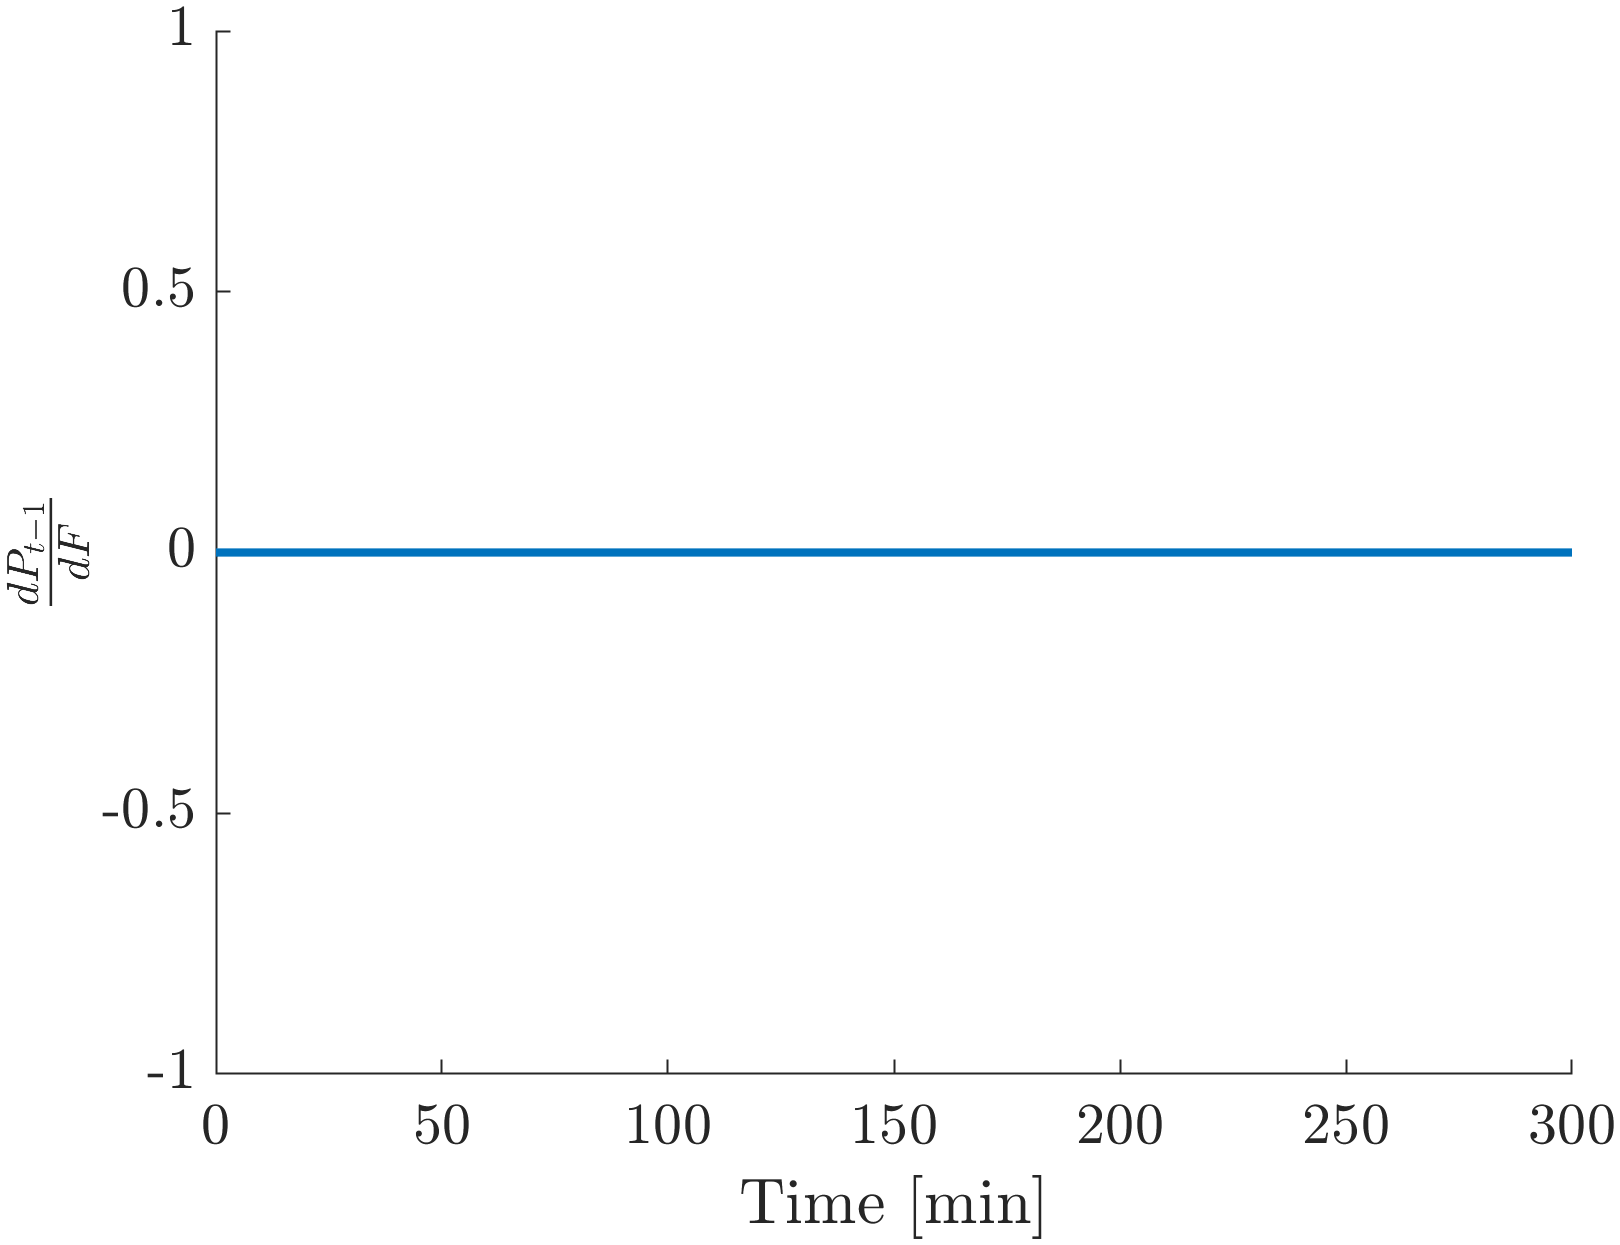
\includegraphics[trim = 0.0cm 0.0cm 0.0cm 0.0cm,clip,width=\columnwidth]{/Results_sensitivity/P_F.png}
		\caption{The effect of $F$ change on $P$}
		\label{fig:Sensitivty_F_P}
	\end{figure}
	
	It is important to note that $h$ represents enthalpy but not total enthalpy, thus excluding kinetic energy. As a consequence of the modelling assumptions, changes in $h$ and $\rho$ occur in response to changes in pressure or temperature, which explains no deviation of $h \times \rho$ in Figure \ref{fig:Sensitivty_F_H}.
    
    %When utilizing Dirichlet boundary conditions, it's crucial to be aware of potential numerical artefacts from the differing methods used to compute them. The system's enthalpy is determined through the time evolution of governing equations, while the inlet's enthalpy depends on the inlet temperature and pressure, which are the controls. A minor numerical mismatch between these values may manifest as an enthalpy difference propagating along the spatial domain. To ensure consistency between the fluid at the inlet and inside the computational domain, this analysis employs Neumann boundary conditions.
        
    \begin{figure}[h!]
    	\centering
    	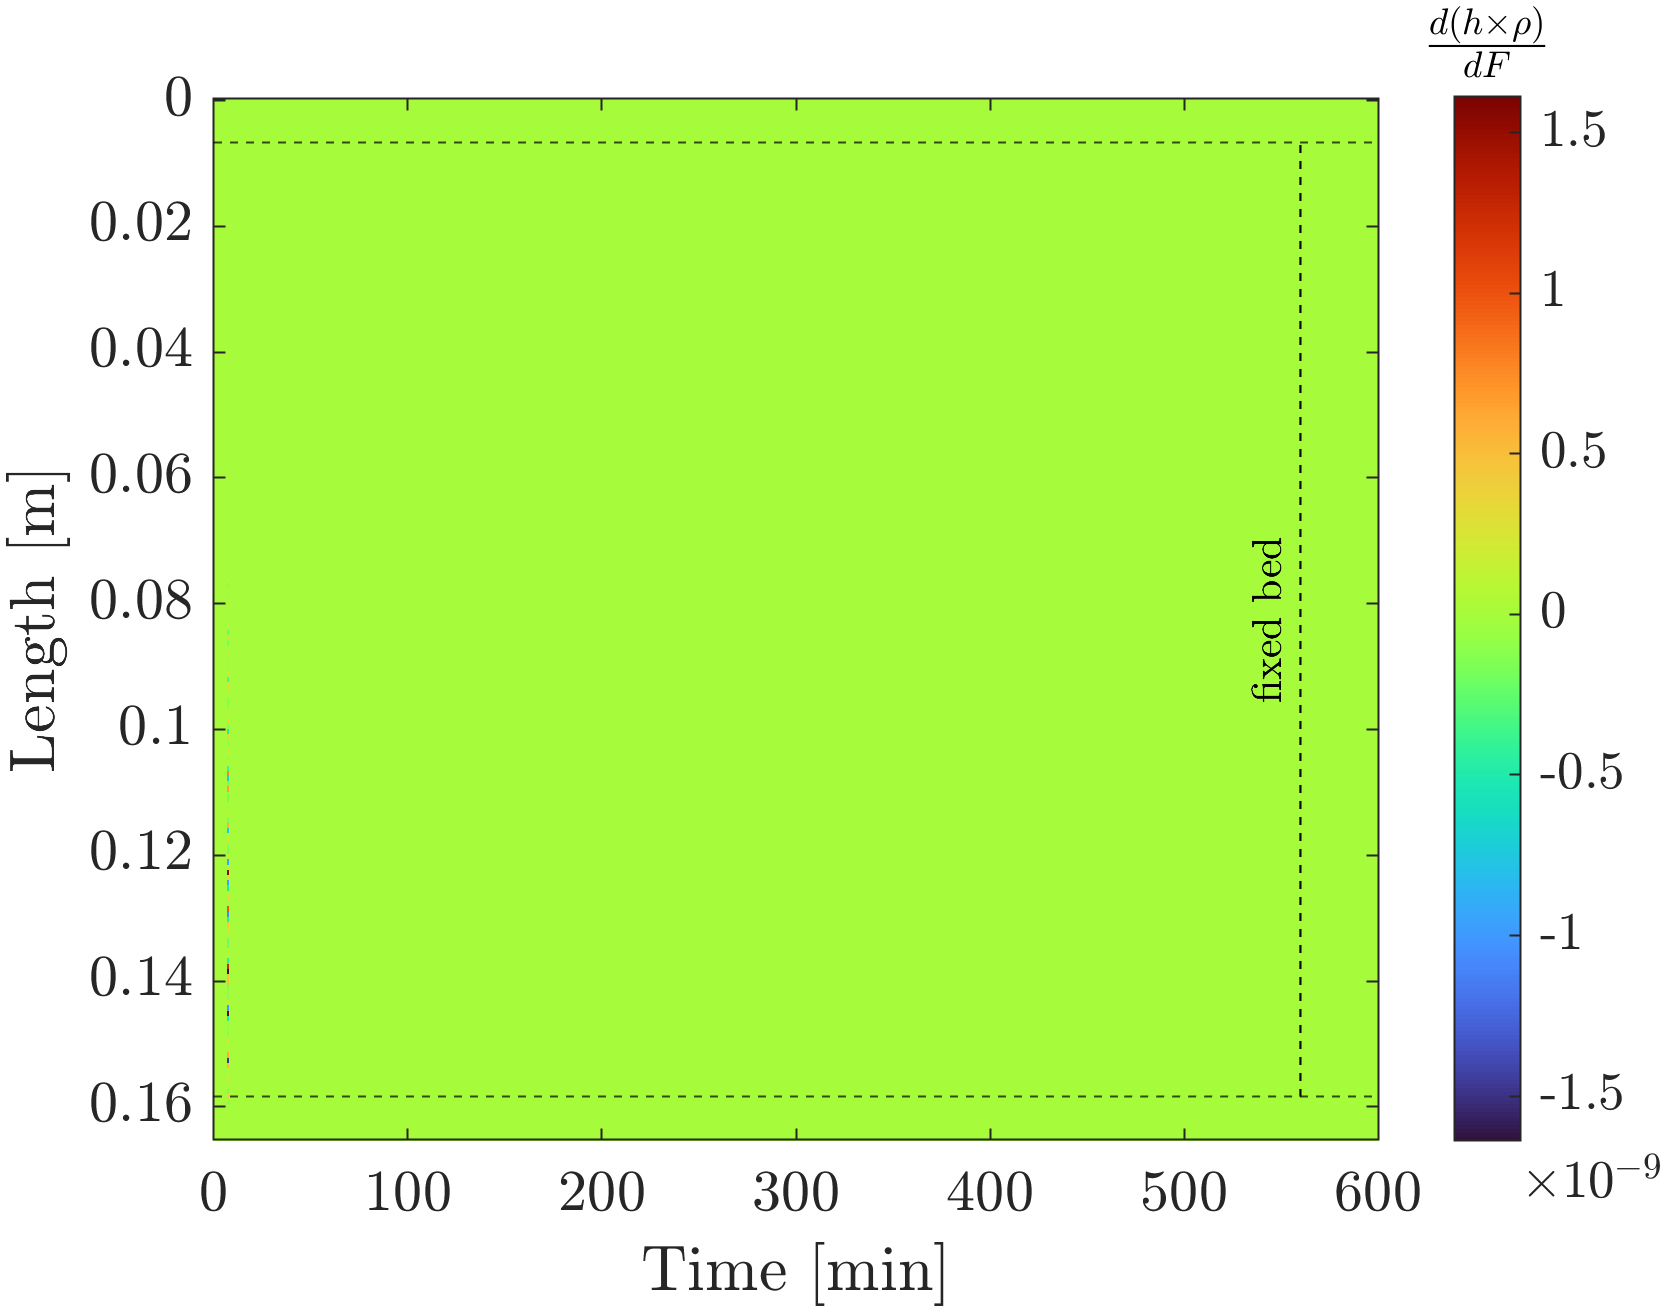
\includegraphics[trim = 0.0cm 0.0cm 0.0cm 0.0cm,clip,width=\columnwidth]{/Results_sensitivity/H_F.png}
    	\caption{The effect of $F$ change on $h \times \rho$}
    	\label{fig:Sensitivty_F_H}
    \end{figure}
   
   Figure \ref{fig:Sensitivty_F_CS} visualizes the local sensitivity of the solute concentration in the solid phase to changes in the mass flow rate during a supercritical fluid extraction process. It is postulated that with an increase in the mass flow rate, the driving force for mass transfer—the concentration gradient—becomes more pronounced, leading to an accelerated decrease in solute concentration within the solid matrix. This is exhibited by the negative sensitivity values: the solute is depleted more rapidly from the solid phase with higher mass flow rates. The most significant sensitivity is seen at the process commencement, particularly at the column inlet (top left corner with bright colours), where the concentration of solute is highest, and the effect of mass flow rate on extraction is most pronounced.
   
   As the extraction progresses, the sensitivity values become less negative, moving towards zero, depicted by the gradient transitioning to cooler colors towards the bottom of the figure. This gradual change corresponds to the decreasing concentration of the solute in the solid phase, which results in a diminishing concentration gradient and, consequently, a reduction in the rate of extraction. The sensitivity approaching zero suggests that the driving force for mass transfer is decreasing as the solute is being depleted.
   
   The asymptotic approach to zero sensitivity indicates a physical plateau in the extraction process, where further increases in mass flow rate no longer enhance the extraction efficiency. In practical terms, this asymptotic behavior signifies the approach towards an extraction endpoint where the remaining solute concentration in the solid phase is minimal and becomes less dependent on the mass flow rate. At this stage, other factors, such as diffusion within the solid matrix or equilibrium limitations, may limit the extraction rate.
   
   In the most extreme cases, depicted by the uniform regions in the plot, the solute has been effectively exhausted, and the remaining traces in the solid phase are no longer influenced by changes in the mass flow rate. This stage represents the final equilibrium, where the concentration gradient effectively drops to zero, rendering the mass flow rate inconsequential for the extraction of the remaining solute. At this juncture, the system has reached its thermodynamic limit, and the efficiency of extraction cannot be enhanced by merely increasing the flow rate. This underscores the importance of optimizing the mass flow rate at the beginning and throughout the extraction process to ensure efficient solute recovery before reaching this terminal stage.
   
   %Figure \ref{fig:Sensitivty_F_CS} shows how the flow rate affects the solute concentration in the solid phase. At the beginning of the extraction process, the flow rate has a low impact on the extraction process due to the dominance of the concentration gradient in the kinetic regime. The corresponding sensitivities are close to zero. As time progresses, the increment in the mass flow rate has a greater influence on the extraction kinetics, causing the sensitivities to decrease towards their minimum values. Negative sensitivities indicate a faster extraction rate. 
    
    \begin{figure}[h!]
    	\centering
    	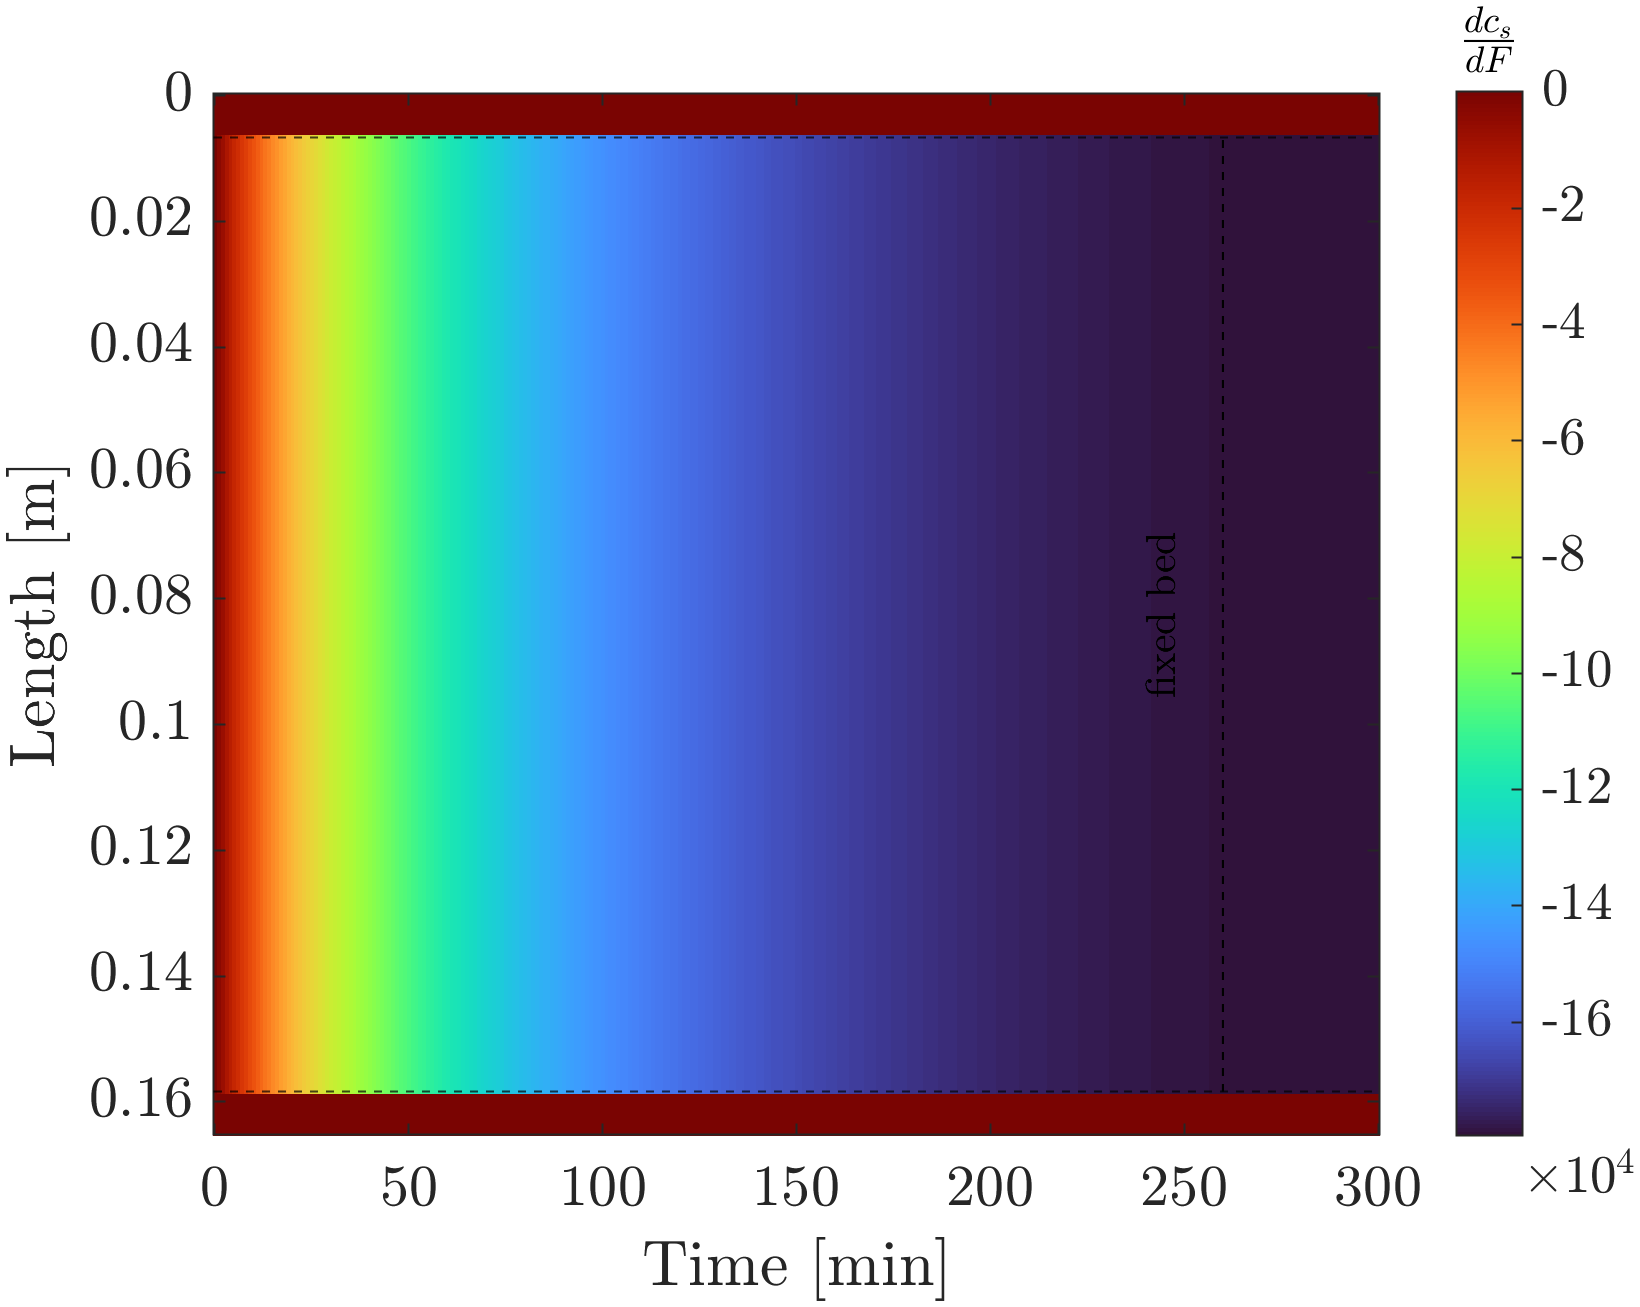
\includegraphics[trim = 0.0cm 0.0cm 0.0cm 0.0cm,clip,width=\columnwidth]{/Results_sensitivity/CS_F.png}
    	\caption{The effect of $F$ change on $C_s$}
    	\label{fig:Sensitivty_F_CS}
    \end{figure}
    
    
    The Figure \ref{fig:Sensitivty_F_CF} depicts the sensitivity of the solute concentration in the fluid phase to the flow rate within a supercritical fluid extraction system. This sensitivity analysis reveals how the solute's behavior in the fluid phase is influenced by variations in the flow rate over the course of the extraction process, as depicted by both time and the length of the extraction column.
    
    In the initial phase of the extraction, the sensitivities near the inlet are negligible, as shown by the colors being close to zero. This indicates a minimal initial response to changes in the flow rate, which could be due to the presence of an high concentration gradient, allowing the fluid phase to rapidly reach solute regardless of the flow rate.
    
    As the extraction progresses, positive sensitivities emerge along the length of the extractor, indicated by the concentration front that develops and moves along the flow direction. This front represents the increased movement of the solute with the fluid phase as the flow rate increases, suggesting an enhanced mass transfer due to the elevated velocity of the supercritical fluid. This velocity increase augments the concentration gradient, thus encouraging a more efficient solute migration from the solid to the fluid phase.
    
    Following the positive front, there is an emergence of a front characterized by negative sensitivities. This trend illustrates a diminishing solute concentration in the fluid phase, and it reflects a point in the extraction where the solute availability in the solid phase becomes a limiting factor; the depletion of solute reduces the concentration gradient, thereby decelerating the extraction rate. 
    
    Toward the end of the extraction process, the sensitivities are shown to increase from their negative values towards zero. This asymptotic approach suggests that the system is reaching a kinetic regime where further increases in the flow rate have a low impact on the solute concentration in the fluid phase. This behavior reflects a physical limit where the remaining solute in the solid phase is insufficient to sustain a high concentration in the fluid phase, regardless of the flow rate. It indicates a terminal phase of the extraction process where the available solute has been largely exhausted, and the system response to changes in flow rate is inherently constrained by the depletion of extractable material.
    
    %Figure \ref{fig:Sensitivty_F_CF} shows how the concentration of solute in the fluid phase responds to an increase in the flow rate. Initially, sensitivities are close to zero, indicating a minimal system response. The growth in flow rate affects $C_f(z,t)$ indirectly by increasing the velocity and consequently elevating the concentration gradient. As a result, positive sensitivities emerge within the system, forming a front that progresses in the direction of flow. The positive front indicates that the larger amount of solute moves faster across the system. When the amount of the solute in the solid phase becomes a limiting factor, then the concentration gradient diminishes and slows down the extraction kinetics. The corresponding sensitivities form a front composed of negative sensitivities propagating through the extractor. The negative front indicates that the solute concentration in the fluid phase becomes lower than before the flow rate increment. Eventually, the negative sensitivities start to increase and asymptotically approach zero.
    
    \begin{figure}[h!]
    	\centering
    	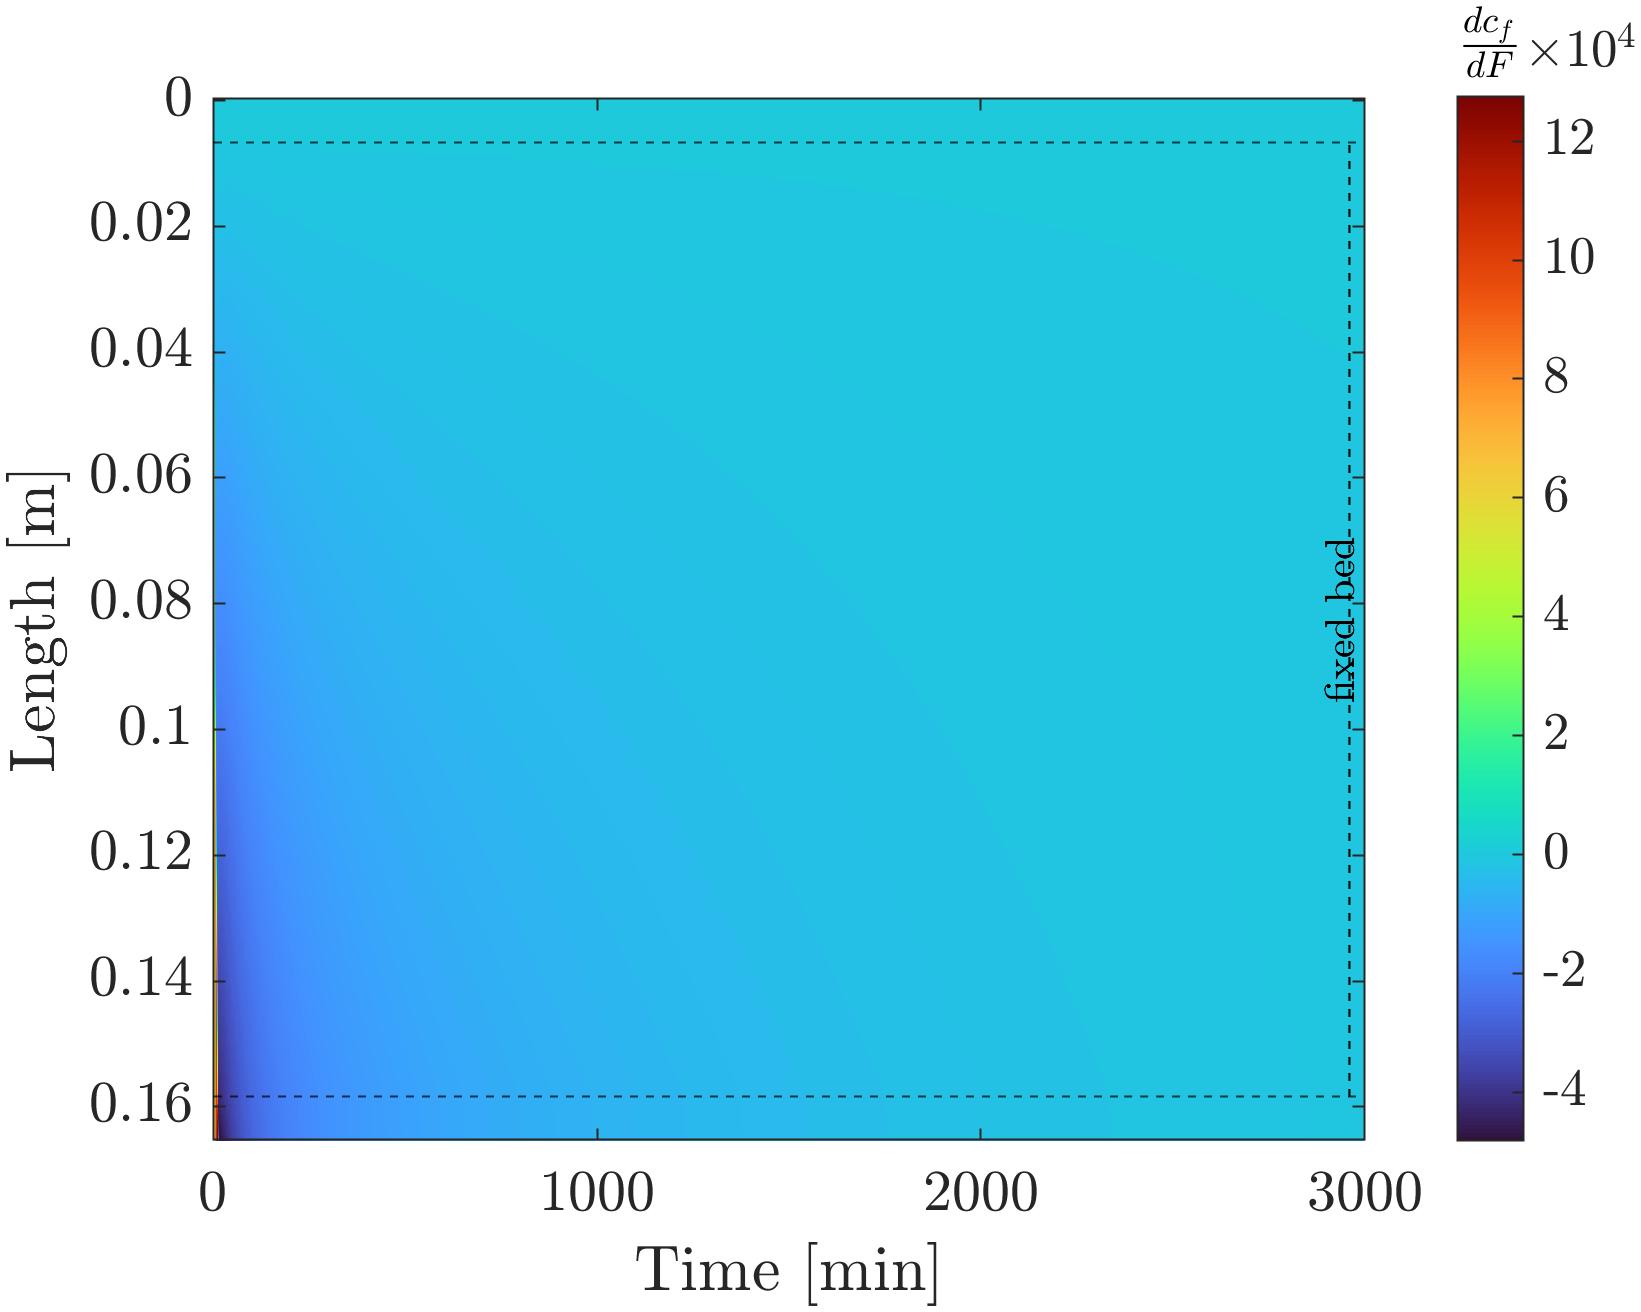
\includegraphics[trim = 0.0cm 0.0cm 0.0cm 0.0cm,clip,width=\columnwidth]{/Results_sensitivity/CF_F.png}
    	\caption{The effect of $F$ change on $C_f$}
    	\label{fig:Sensitivty_F_CF}
    \end{figure}

	
	The Figure \ref{fig:Sensitivty_F_y} depicts the sensitivity of the extraction yield to variations in mass flow rate  as a function of time. The curve’s initial rise to a peak followed by a decline conveys the dynamic relationship between the mass flow rate and the extraction yield within the supercritical extraction process.
	
	In the early phase, the sensitivity is minimal, denoting that adjustments to the mass flow rate have a negligible influence on the yield. This can be attributed to the initial phase of the extraction, where the mass transport mechanisms are mainly controlled by a high concentration gradient.
	
	As the process evolves, the curve's ascent to its apex signifies a period during which the extraction yield becomes increasingly sensitive to the mass flow rate. This is likely due to the mass flow rate enhancing the convective transport of solute, maximizing the extraction efficiency. At this stage, the solute transfer from the solid to the fluid phase is most responsive to changes in flow rate.
	
	However, the curve’s descent past the peak suggests a diminishing return on sensitivity with further increases in mass flow rate. The decrease indicates a transitional phase where the extraction process likely encounters diffusion limitations or a depletion of readily extractable solute. The concentration gradient, which drives the mass transfer, may be reduced due to the depletion of solute in the solid phase, or the system may be experiencing diffusive resistances that limit the rate at which solute can be delivered to the fluid phase.
	
	The asymptotic approach to zero sensitivity towards the end of the curve reflects a regime where the yield is no longer significantly influenced by the mass flow rate. At this juncture, the extraction process has likely exhausted the available solute, and any further increase in mass flow rate does not result in a proportional increase in yield. The extraction system has reached a point of saturation or equilibrium where the mass transfer is limited by factors other than flow rate, such as the intrinsic properties of the solute or the matrix, indicating that the system has achieved as much extraction as is practically feasible under the given conditions.
	
	The curve captures the non-linear and transient nature of the extraction yield's response to the mass flow rate, underscoring the importance of optimizing flow rates over the duration of the extraction to maximize yield. It also highlights the multifaceted dependencies and constraints inherent in supercritical fluid extraction processes, such as mass transfer rates, solute availability, and diffusion limitations.

    %In Figure \ref{fig:Sensitivty_F_y}, the curve's shape reveals the time-dependent sensitivity of extraction yield to mass flow rate variations. The curve peaks and then falls, indicating a transient behavior in extraction efficiency. Initially, there's a negligible response, suggesting that changes in mass flow rate have little to no immediate impact on yield. As time progresses, however, yield becomes increasingly sensitive to the flow rate, reaching a peak sensitivity. Beyond this peak, the sensitivity decreases, which might reflect a saturation point in the extraction process where further increases in mass flow rate do not translate to increased yield, possibly due to limitations in solute diffusion rates from the solid matrix and decreasing concentration gradient. Eventually, $dy/dF$ asymptotically approaches zero. This happens because the amount of solute in the fluid phase becomes a limiting factor, and the process is in the diffusion regime.
    
    \begin{figure}[h!]
    	\centering
    	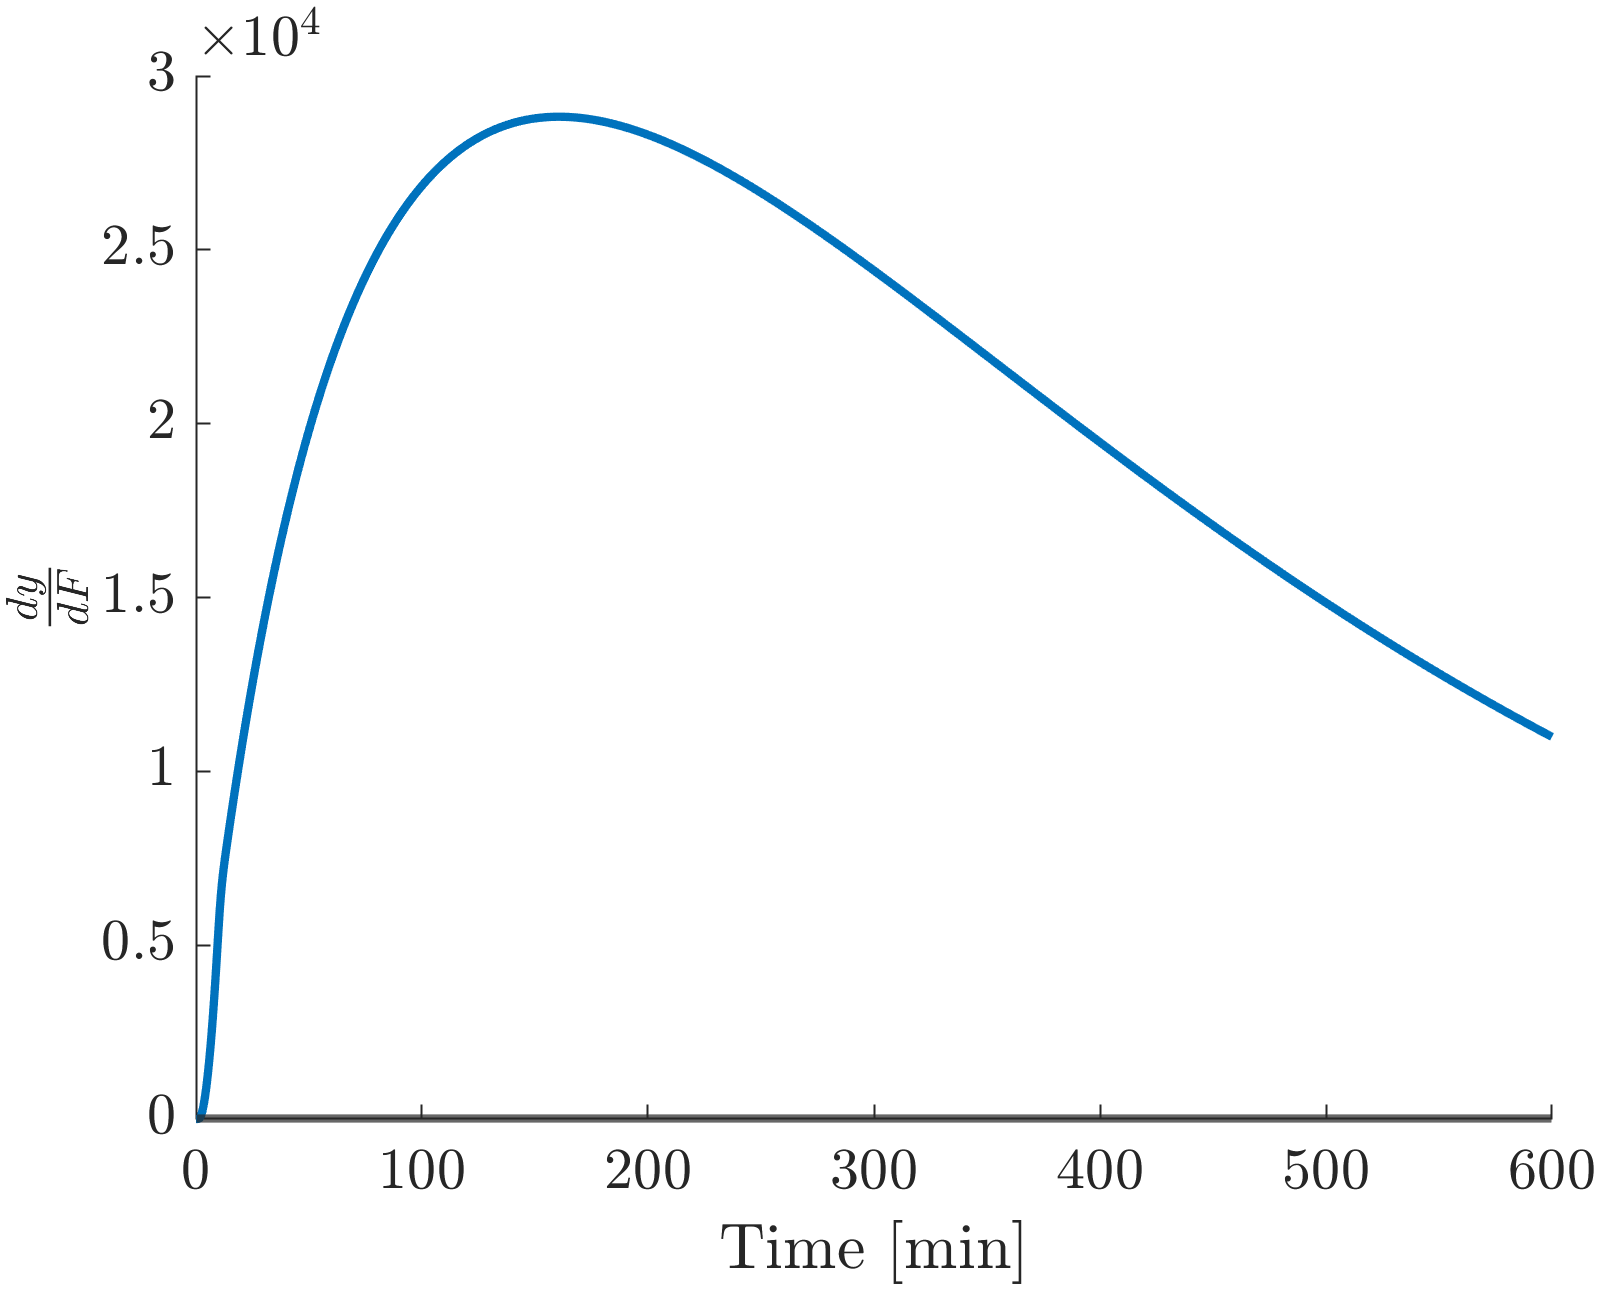
\includegraphics[trim = 0.0cm 0.0cm 0.0cm 0.0cm,clip,width=\columnwidth]{/Results_sensitivity/Y_F.png}
    	\caption{The effect of $F$ change on $y(t)$}
    	\label{fig:Sensitivty_F_y}
    \end{figure}
    
    \subsection{Pressure}
    
    As discussed in Chapter \ref{CH:Governing_equations_chapter}, a small pressure wave propagates at the speed of sound relative to the flow. If the flow velocity is relatively low, all pressure changes are hydrodynamic (resulting from velocity motion) rather than thermodynamic. The Low Mach-number assumption leads to instant propagation of the thermodynamic pressure throughout the system. This assumption allows considering a single pressure value for the entire system, as all changes occur simultaneously within the machine. Figure \ref{fig:Sensitivty_P_P} illustrates a step function representing the pressure change.
    
    \begin{figure}[h!]
    	\centering
    	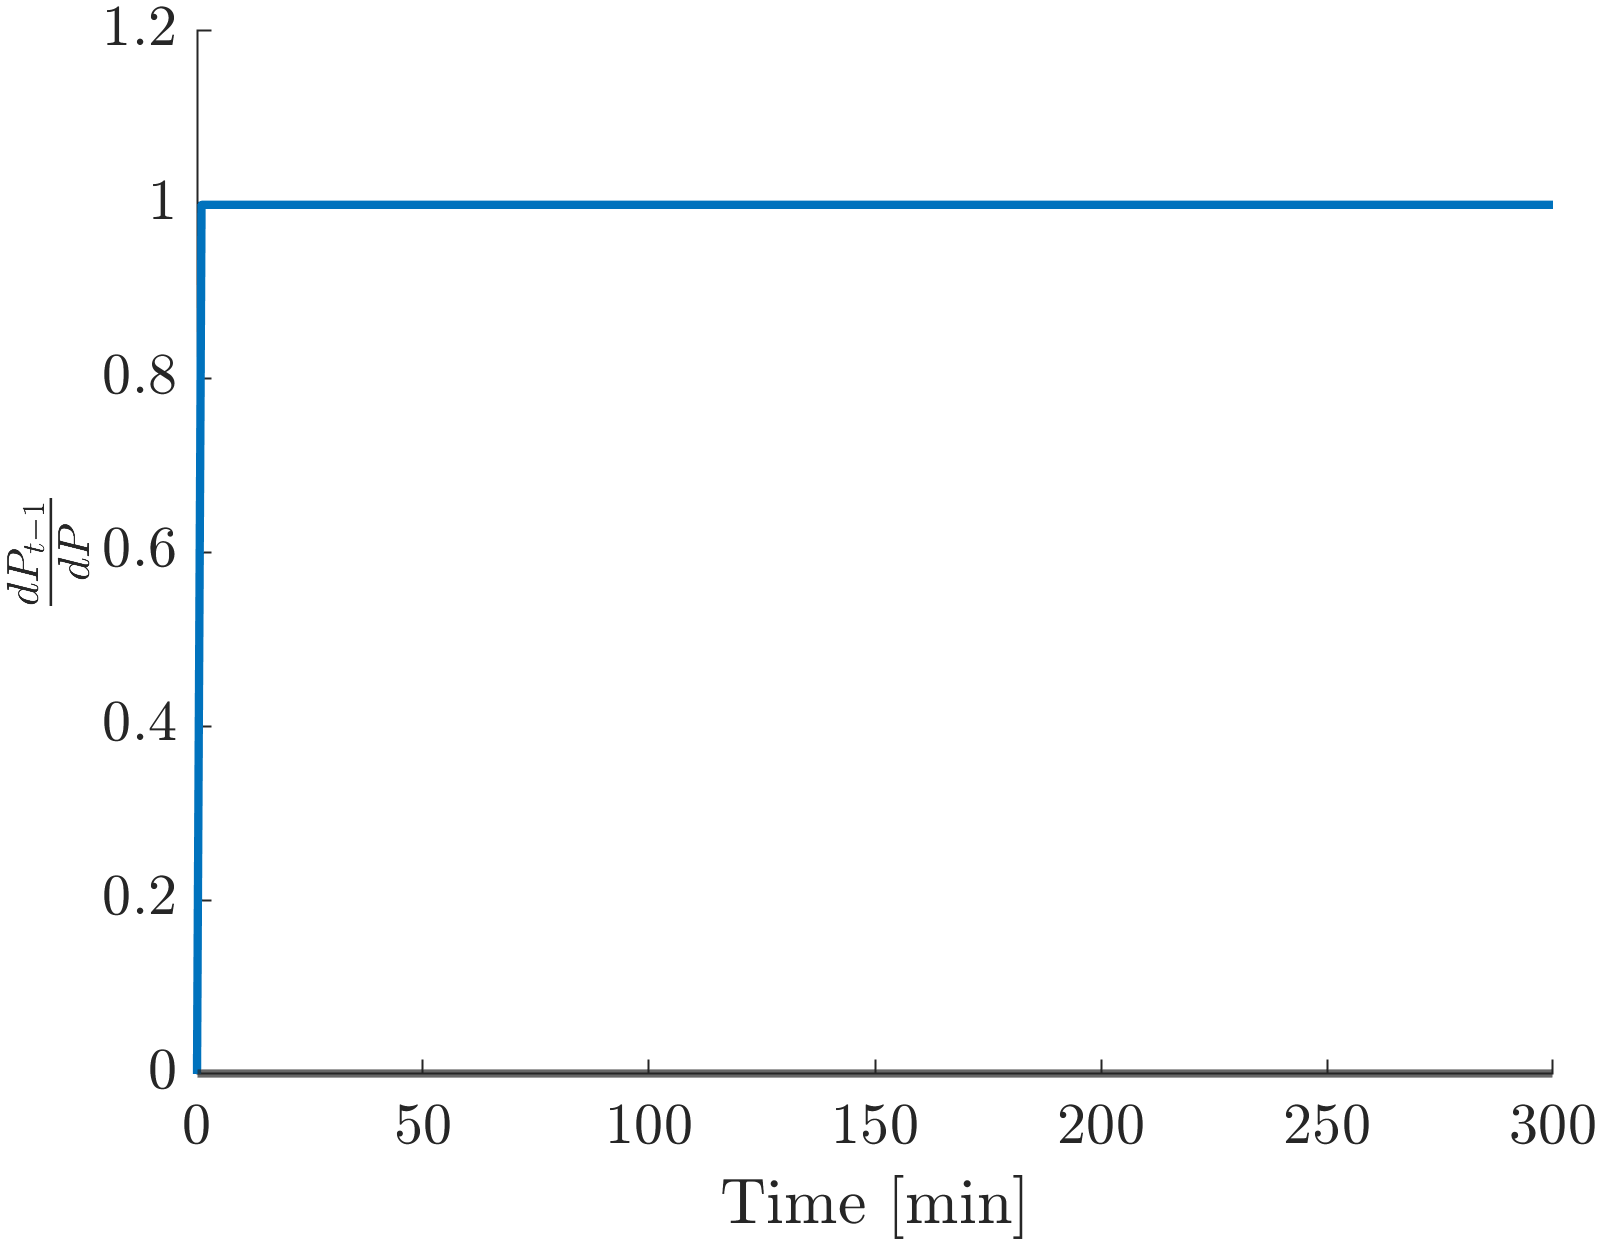
\includegraphics[trim = 0.0cm 0.0cm 0.0cm 0.0cm,clip,width=\columnwidth]{/Results_sensitivity/P_P.png}
    	\caption{The effect of $P$ change on $P$ in the system}
    	\label{fig:Sensitivty_P_P}
    \end{figure}
    
    According to Equation \ref{EQ:Enthalpy_equation}, the pressure change directly affects the quantity $h \times \rho$ through $\partial (P(t) A_f) / \partial t$, leading to the step change along the whole system, as presented in Figure \ref{fig:Sensitivty_P_H}. The uniform response across the entire extraction column length and time, represented by the homogeneously dark red color, indicates that the entire system experiences an immediate and uniform change in enthalpy density in response to pressure changes. This is consistent with the physical expectation that pressure changes should equilibrate rapidly throughout the fluid phase due to the high compressibility of supercritical fluids.
    
    Regarding the boundary conditions, by applying the Dirichlet boundary conditions( mean setting a fixed temperature at the system boundary) can leads to a possible thermal gradient within the system if the initial temperatures differ. In contrast, Neumann boundary conditions would dictate that the heat flux at the boundaries be held constant, ensuring temperature uniformity between the inlet and the rest of the extractor. In case of this work, the Neumann boundary conditions have been applied, as indicated by the uniform response in enthalpy density, implying that there is no temperature gradient caused by a heat front propagating through the system. Instead, the temperature within the extractor is instantaneously and evenly matched to that at the inlet.
    
	%According to Equation \ref{EQ:Enthalpy_equation}, the pressure change directly affects the quantity $h \times \rho$ through $\partial (P(t) A_f) / \partial t$, leading to the step change along the whole system, as presented in Figure \ref{fig:Sensitivty_P_H}. Depending on the configuration of the system, two cases are possible. If Dirichlet boundary conditions are applied, the inlet temperature is maintained at the predefined value and may differ from the temperature in the extractor. In such a case, the temperature difference will cause the heat front to propagate through the system. Alternatively, Neumann boundary conditions can be applied to ensure that the temperature inside the extractor matches that at its inlet. In this work, the second approach was chosen.
    
    \begin{figure}[h!]
    	\centering
    	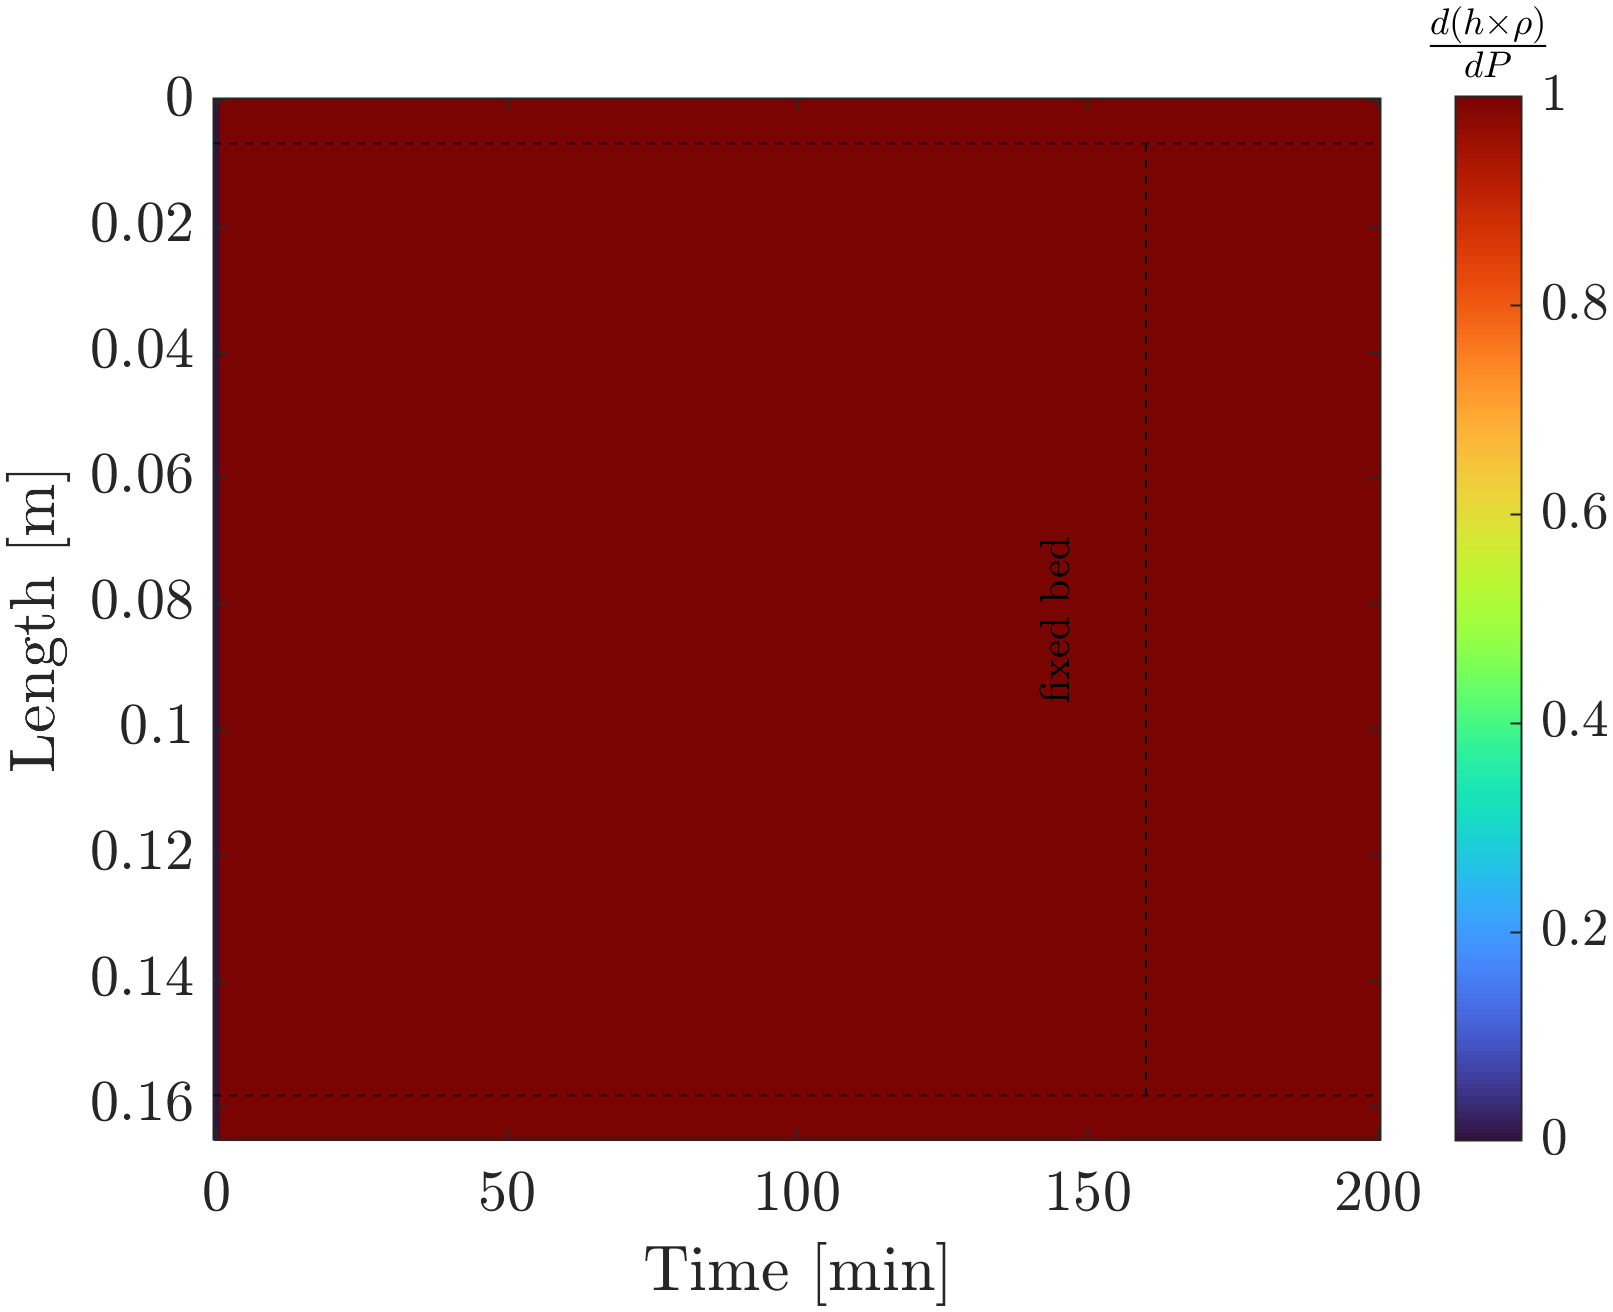
\includegraphics[trim = 0.0cm 0.0cm 0.0cm 0.0cm,clip,width=\columnwidth]{/Results_sensitivity/H_P.png}
    	\caption{The effect of $P$ change on $(h \times \rho)$ in the system}
    	\label{fig:Sensitivty_P_H}
    \end{figure}
    
    The provided figure showcases the sensitivity of the solute concentration in the solid phase with respect to changes in pressure throughout a fixed bed in a supercritical fluid extraction process. 
    
    As discussed in Chapter \ref{CH: Continuity}, the velocity of a fluid is inversely related to its density, which suggests that with higher fluid density—often associated with increased pressure—the velocity decreases. This leads to an extended residence time of the fluid within the system. The lower velocity afforded by increased pressure allows for a longer interaction between the solute and the solvent, potentially a higher concentration of solute in the fluid phase.
    
    Simultaneously, pressure changes alter the fluid's thermodynamic state, affecting the extraction process's kinetics. These changes are characterized by correlations ({\color{red}article 1}), such as the increase of the diffusion coefficient $D_i^R$ with fluid density. A higher $D_i^R$ indicates enhanced mass transfer capabilities, contributing to an increased rate of extraction.
    
    Figure \ref{fig:Sensitivty_P_CS} captures these dual effects on the solute concentration within the solid matrix. Initially, the system response is low due to a high concentration gradient. When the concentration gradient starts to diminish, high sensitivities reveal that changes in pressure have a more pronounced effect. This is consistent with the fluid's higher density and lower velocity, resulting in more effective mass transfer from the solid to the fluid phase.
    
    Over time, the pressure change has a lower effect and the sensitivities decay. This trend signifies that the impact of pressure on solute concentration is diminishing, likely due to the depletion of the solute in the solid phase over time. The decreasing concentration gradient suggests that the solute availability becomes a limiting factor in the extraction process.
    
    Eventually, sensitivities asymptotically approach zero. The solute concentration in the solid phase has been reduced, and further changes in pressure do not influence the remaining concentration. This behaviour reflects that in the later extraction phase, the kinetics of extraction are dominated by the reduced availability of the solute rather than the conditions of the supercritical fluid.

	%The pressure change affects the mass transfer in two ways. As discussed in Chapter \ref{CH: Continuity}, the velocity is inversely proportional to the density; hence, the higher density of the fluid leads to a lower velocity and larger residence time. The changes in the thermodynamic state of the fluid affect the extraction kinetic parameters, which are defined by correlations presented in {\color{red}article 1}. For example, the $D_i^R$ increases with the fluid density, which leads to a higher extraction rate. The cumulative effect of the pressure change on the solute concentration in the solid phase can be observed in Figure \ref{fig:Sensitivty_P_CS}. The sensitivity plot shows a close-to-uniform decay of sensitivities along the fixed bed. After the extremum, the sensitivities asymptotically increase to zero.

	\begin{figure}[h!]
		\centering
		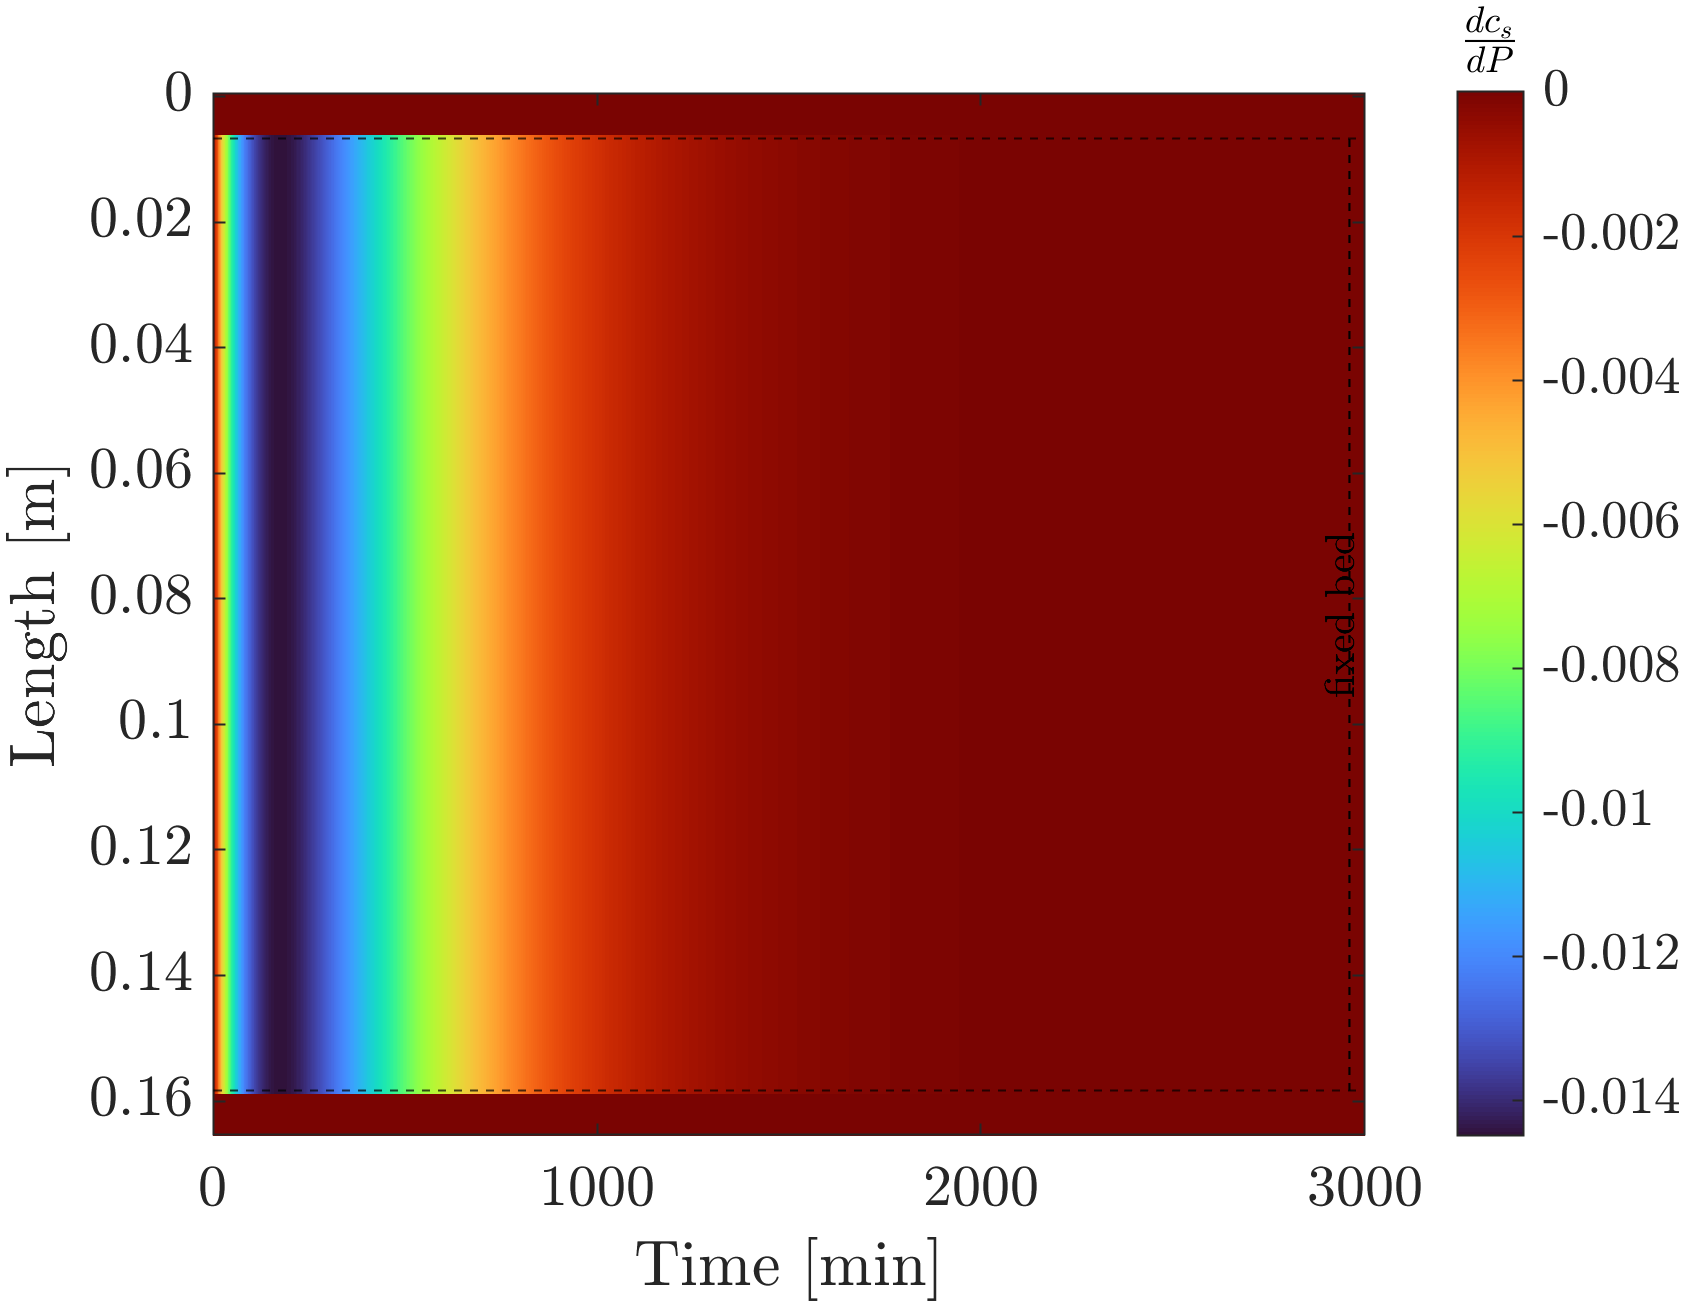
\includegraphics[trim = 0.0cm 0.0cm 0.0cm 0.0cm,clip,width=\columnwidth]{/Results_sensitivity/CS_P.png}
		\caption{The effect of $P$ change on $C_s$}
		\label{fig:Sensitivty_P_CS}
	\end{figure}

	Figure \ref{fig:Sensitivty_P_CF} shows the sensitivity of the solute concentration in the fluid phase as a function of pressure changes throughout the supercritical extraction column's length and over the extraction process's duration. An increase in pressure typically enhances the solute's solubility, resulting in its heightened presence in the supercritical fluid, which is seen as a leading front moving through the system. Due to the diffusion effect, the gradient becomes more dispersed in regions beyond the fixed bed. Following this, the formation of a trailing front characterized by decreasing sensitivities can be observed. This trailing front can be explained by the decrease in the concentration gradient as the solute is increasingly extracted and the available concentration within the solid phase diminishes. As seen in the figure, sensitivities are declining towards zero. This asymptotic trend suggests the driving force for the mass transfer—the concentration gradient—has been minimized, and changes in pressure no longer significantly impact the solute concentration in the fluid phase.

	%The deviation in the solute concentration in the fluid phase caused by the pressure change is presented in Figure \ref{fig:Sensitivty_P_CF}. As discussed earlier, the sensitivities related to the solute concentration in the solid phase are characterized by negative sensitivities, suggesting a higher extraction rate due to the pressure change. Consequently, an increase in solute concentration in the fluid phase is expected. This increase in solute concentration in the fluid phase is visible in Figure \ref{fig:Sensitivty_P_CF} as positive sensitivities, which form a front that moves along the extractor. Due to the diffusion effect, the front changes its pattern in the empty section and becomes more spread. Accelerating the extraction rate since the beginning of the extraction process leads to a faster decrease in the concentration gradient. This effect is reflected in Figure \ref{fig:Sensitivty_P_CF} as the front of the negative sensitivities, which follows the positive front. Eventually, the negative sensitivities approach zero when the concentration gradient goes to zero.

	\begin{figure}[h!]
		\centering
		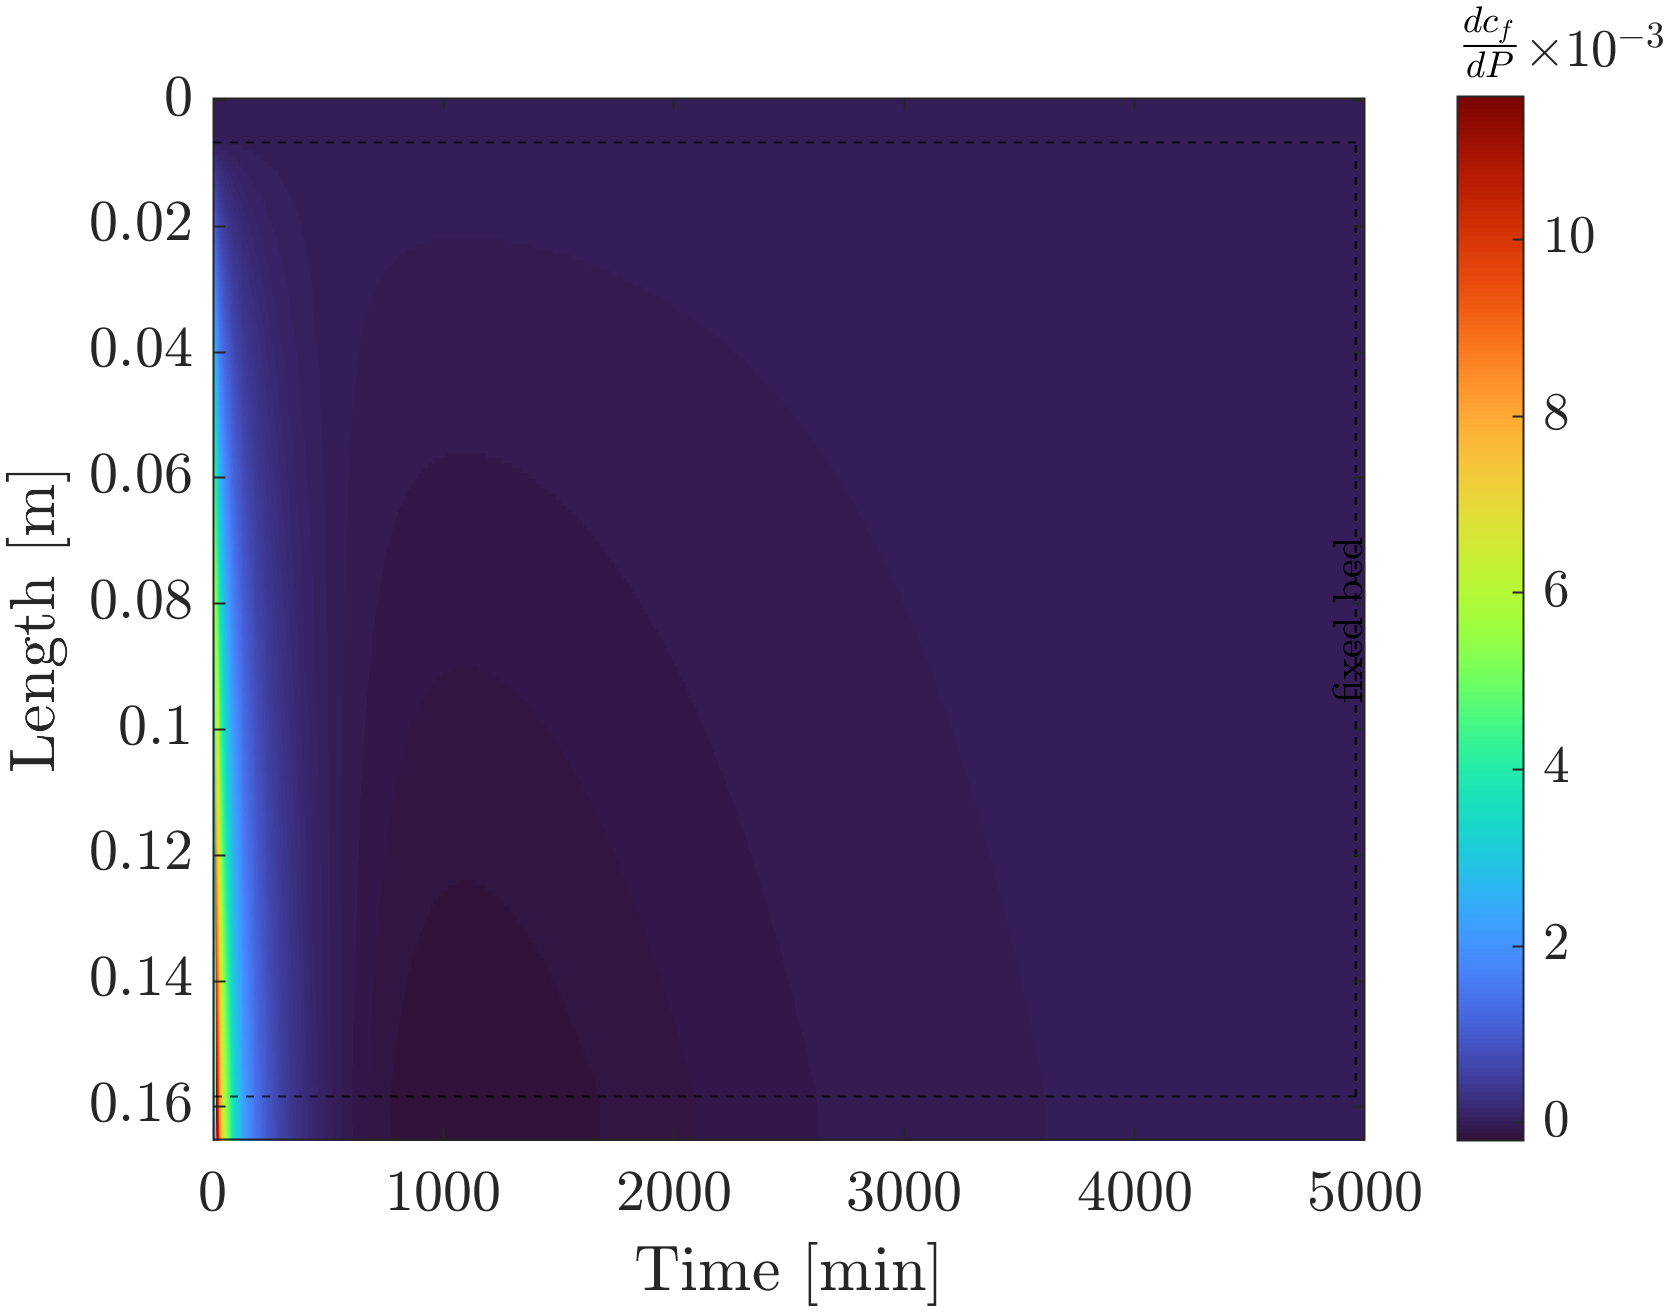
\includegraphics[trim = 0.0cm 0.0cm 0.0cm 0.0cm,clip,width=\columnwidth]{/Results_sensitivity/CF_P.png}
		\caption{The effect of $P$ change on $C_f$}
		\label{fig:Sensitivty_P_CF}
	\end{figure}

	Figure \ref{fig:Sensitivty_P_y} illustrates the temporal evolution of the extraction yield's sensitivity to changes in pressure within a supercritical fluid extraction system. 
	
	Initially, the curve displays an almost flat profile, suggesting a latency in the system's response to pressure changes. A minor initial decrease in sensitivity, indicated by a slight dip below zero, may arise due to a decrease in the velocity of the fluid phase. For a constant mass flow rate, an increase in fluid density due to heightened pressure results in a lower fluid velocity, potentially leading to this reduced sensitivity.
	
	As the process continues, the curve ascends sharply, indicating a positive yield response to pressure. This increase in sensitivity can be associated with the enhanced solubility and mass transfer capabilities imparted by higher pressures, improving the rate at which solute is extracted into the fluid phase. The peak in dy/dP reflects the most responsive period of the system, where pressure changes are highly effective in improving yield.
	
	Beyond the peak, the sensitivity declines, converging towards zero. This descending curve represents a depletion phase: as the available solute in the solid phase diminishes, the potential for further increasing the yield through pressure alone is reduced. The remaining solute concentration becomes a limiting factor, and the mass transfer driving force, initially augmented by pressure, no longer plays a dominant role.

	%The impact of pressure increase on extraction yield is depicted in Figure \ref{fig:Sensitivty_P_y}. The initial flat curve reflects a system delay caused by the empty space within the extractor that the fluid phase needs to flow through. The first observed deviation is a small negative sensitivity, which can be related to a lower fluid phase velocity. Keeping the same mass flow rate and increasing the density (by increasing the pressure) decreases the velocity. Next, the sensitivity rises, which indicates an increase in yield. $dy / dP$ reaches its positive maximum and then declines due to a limited amount of solute remaining in the solid phase. The sensitivity curve draws into negative values, reach a minimum point, and converges to zero. The simulation duration was extended to demonstrate the convergence of $dy / dP$ towards zero.

	\begin{figure}[h!]
		\centering
		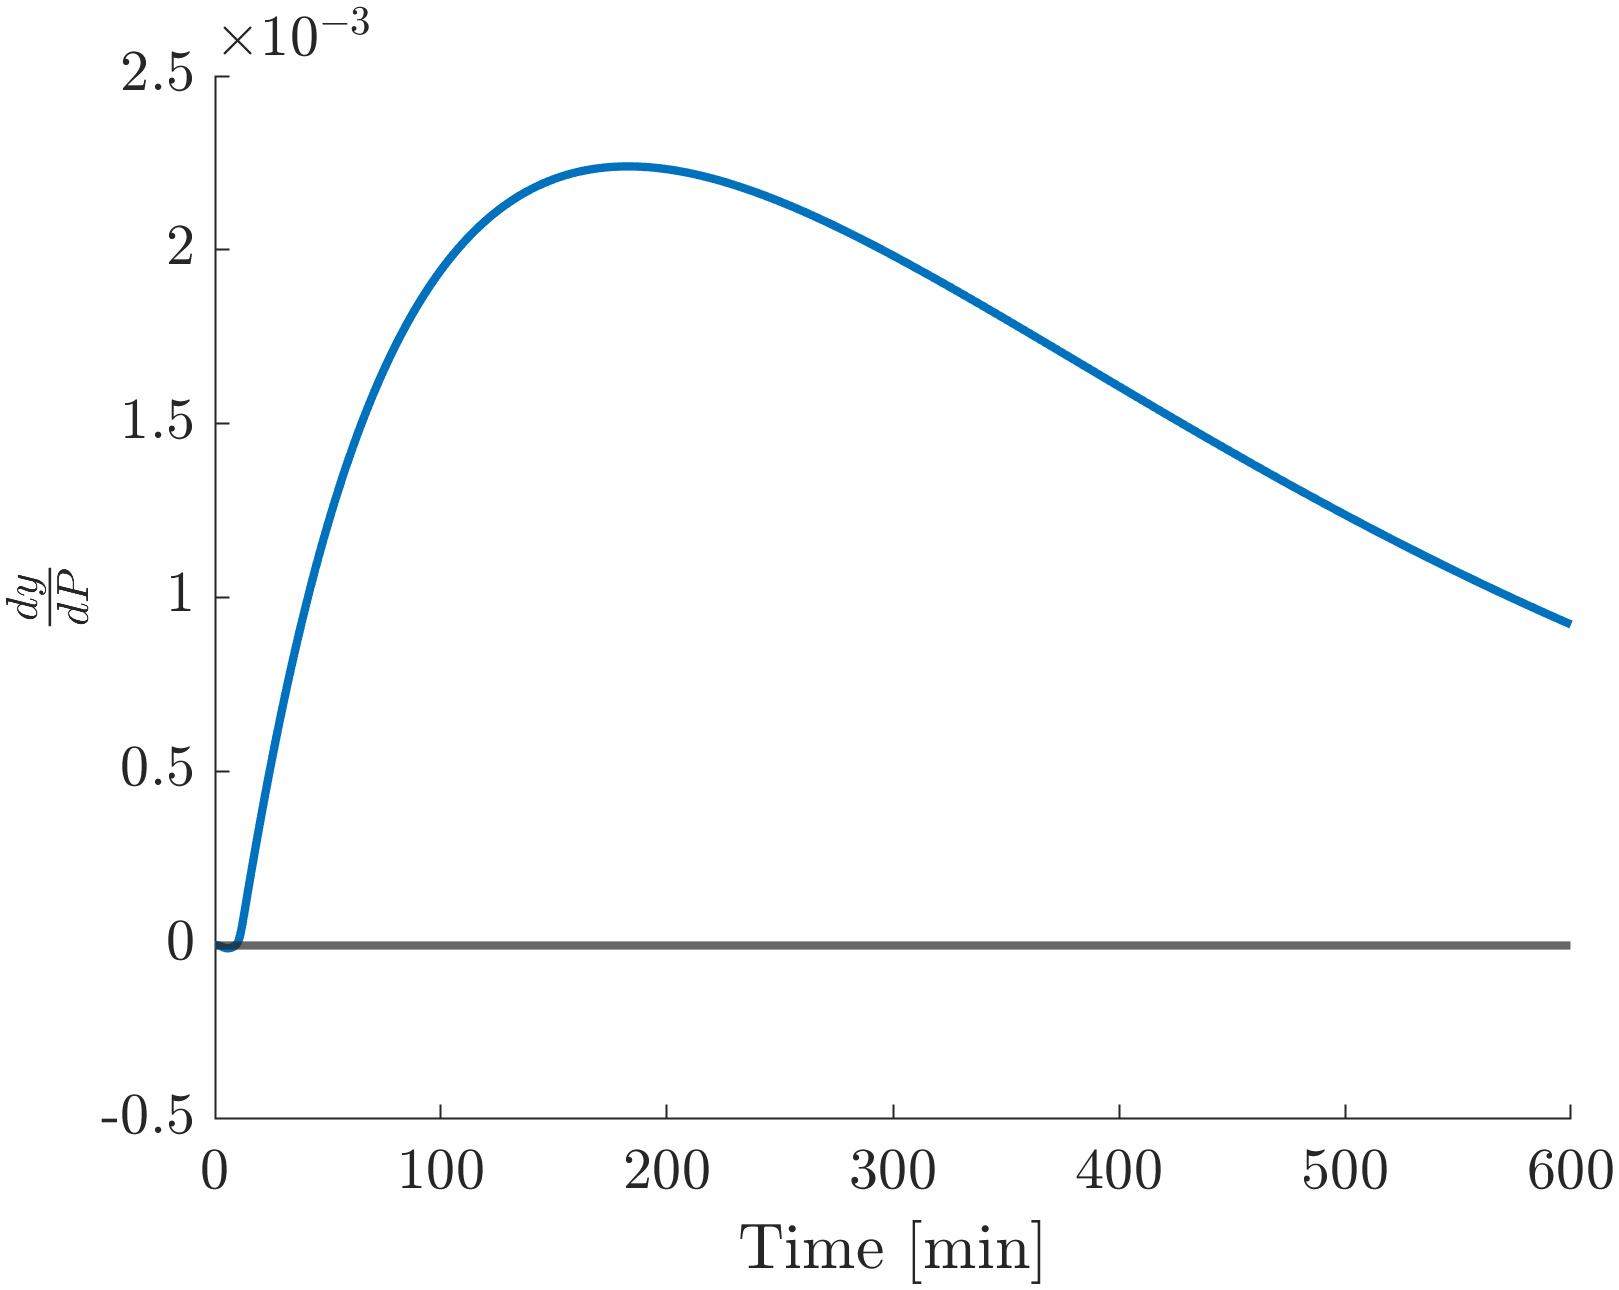
\includegraphics[trim = 0.0cm 0.0cm 0.0cm 0.0cm,clip,width=\columnwidth]{/Results_sensitivity/Y_P.png}
		\caption{The effect of $P$ change on $y(t)$}
		\label{fig:Sensitivty_P_y}
	\end{figure}

	\subsection{Inlet temperature}
	
	The sensitivity analysis of the inlet temperature differs from the two cases presented earlier because the perturbation does not affect the entire system instantaneously; instead, it propagates through it.
	
	The Figure \ref{fig:Sensitivty_P_T} shows the system pressure response. A flat curve indicates an invariant behavior of pressure in response to inlet temperature changes throughout the time. The pressure in the modelled system is controlled and maintained independently of the inlet temperature variations as a results of the assumptions as explained in the Chapter X.
	%The sensitivity analysis of the inlet temperature differs from the two cases presented earlier because the perturbation does not affect the entire system instantaneously; instead, it propagates through the system. As the fluid with the modified temperature flows along the system, it gradually modifies the mass transfer parameters. One important assumption is that the inlet temperature change does not affect the pressure, which explains a horizontal line in Figure \ref{fig:Sensitivty_P_T}.
	
	\begin{figure}[h!]
		\centering
		\includegraphics[trim = 0.0cm 0.0cm 0.0cm 0.0cm,clip,width=\columnwidth]{/Results_sensitivity/P_T_{in}.png}
		\caption{The effect of $T_{in}$ change on $P$ in the system}
		\label{fig:Sensitivty_P_T}
	\end{figure}

	The inlet enthalpy is characterized by the Dirichlet boundary condition. The boundary value of $(h\times \rho)$ is calculated based on two controls which can be manipulated: inlet temperature and given pressure. Any deviation in $T_{in}$ affects $(h\times \rho)$ at the inlet, propagating according to the governing equations.
	Figure \ref{fig:Sensitivty_T_H} showcases the sensitivity of the fluid enthalpy to the inlet temperature over both time and the length of the extraction bed. The fluid entering the extraction bed will have its enthalpy directly influenced by the boundary conditions. The heat front propagation from the inlet of the extractor to its outlet. As the fluid progresses through the bed, the enthalpy change affects the whole system gradually. Over time, the system's approach to a new thermal steady state and the sensitivities becomes zero.
	
	%The heat front propagation is presented in Figure \ref{fig:Sensitivty_T_H}. The initial system had constant temperature along the whole spatial domain. 
	
	\begin{figure}[h!]
		\centering
		\includegraphics[trim = 0.0cm 0.0cm 0.0cm 0.0cm,clip,width=\columnwidth]{/Results_sensitivity/H_T_{in}.png}
		\caption{The effect of $T_{in}$ change on $(h \times \rho)$ in the system}
		\label{fig:Sensitivty_T_H}
	\end{figure}

	Figure \ref{fig:Sensitivty_T_CS} shows the curve depicts an initial increase (the positive sign of the sensitivities) in the solute concentration in the solid phase as a function of time, which later asymptotically approaches a stable value before decreasing again towards the end of the period. Although $D_i^R$ decreases with the fluid's density, the $\Upsilon$ increases, which explains the system responses. This suggests that an increase in temperature slows the mass transfer of solutes from the solid phase to the supercritical fluid; hence, the solute concentration in the solid phase increases. Over time, this effect stabilizes, which could indicate the exhaustion of easily extractable solutes.
	%Figure \ref{fig:Sensitivty_T_CS} illustrates how the change in inlet temperature affects the concentration of solute in the solid phase. As presented in {\color{red}article 1}, the value of $D_i^R$ decreases as density decreases. Therefore, it is expected to observe positive sensitivities in Figure \ref{fig:Sensitivty_T_CS}, indicating a slower extraction rate. Initially, the sensitivities are zero along the fixed bed because the heat front requires time to reach the fixed bed. Since this propagation is not instantaneous, a non-uniform distribution of sensitivities along the fixed bed becomes evident. All the sensitivities gradually increase until they reach their maximum. When the concentration gradient becomes the limiting factor, the sensitivities decrease.

	\begin{figure}[h!]
		\centering
		\includegraphics[trim = 0.0cm 0.0cm 0.0cm 0.0cm,clip,width=\columnwidth]{/Results_sensitivity/CS_T_{in}.png}
		\caption{The effect of $T_{in}$ change on $C_s$ in the system}
		\label{fig:Sensitivty_T_CS}
	\end{figure}

	The Figure \ref{fig:Sensitivty_T_CF} represents the sensitivity of the concentration of solutes in the fluid phase over a period of 600 minutes as a result of changes in the inlet temperature. Initially, all the sensitivities remain at zero due to the idle period. As the fluid with elevated temperature flows through the fixed bed, the internal mass transfer slows down (the $D_i^R$ is proportional to density as presented in {\color{red}article 1}), resulting in negative sensitivities. The negative sensitivities can be explained by considering that the heat front slowed mass transfer, causing more solute to remain in the solid phase. After reaching their minima, the sensitivities increase and reach positive values. Later the sensitivities starts to increase due higher concentration gradient if compared to before the temperature change. Eventually, the system response stabilize around a constant value when the extraction kinetics become a limiting factor.
	
	\begin{figure}[h!]
		\centering
		\includegraphics[trim = 0.0cm 0.0cm 0.0cm 0.0cm,clip,width=\columnwidth]{/Results_sensitivity/CF_T_{in}.png}
		\caption{The effect of $T_{in}$ change on $C_f$ in the system}
		\label{fig:Sensitivty_T_CF}
	\end{figure}

	Figure \ref{fig:Sensitivty_T_y} depicts how an increase in inlet temperature alters the extraction yield. Initially, the sensitivity curve remains flat due to the idle time. The first observed response of the system is a small increment of the $dy/dT_{in}$ caused by an increment of the velocity( which is inversely proportional to the fluid density). After the small positive peak, the sensitivity curve begins to decrease. The negative value of the sensitivity indicates a lower process efficiency. Over time, the sensitivity reaches its minimum and then increases due to a higher concentration gradient than in the case without the disturbance. Eventually, the $dy/dT_{in}$ curve flattens around a negative value. The flattening of the yield curve suggests that the mass transfer parameters limit the extraction rate, and the residual solute in the solid phase becomes difficult to obtain. The simulation time was extended to show how the sensitivity plot flattened.

	\begin{figure}[h!]
		\centering
		\includegraphics[trim = 0.0cm 0.0cm 0.0cm 0.0cm,clip,width=\columnwidth]{/Results_sensitivity/Y_T_{in}.png}
		\caption{The effect of $T_{in}$ change on $y(t)$ in the system}
		\label{fig:Sensitivty_T_y}
	\end{figure}
	
\end{document}


































